\documentclass{article}
\usepackage{amsmath}
\usepackage{amssymb}
\usepackage{graphicx}
\begin{document}
	\section[Square]{Square Wave}
	A repeating (cyclic) square wave with a frequency of $f$ Hertz and an 
	amplitude of $V$ Volts can be given by the following function.  Let $u(t)$ 
	be defined as the unit step function and $g(t)$ be defined as:
	$$ g(t) := V\Big(2u\big(\sin (2 \pi f t)\big) - 1\Big)$$
	It can also be approximated by the (Fast) Fourier Transform (FFT).
	\subsection[FFT]{Fast Fourier Transform}
	Let $m := 2i + 1$ and let $h(t \vert n)$ be defined as:
	$$ h(t\vert n) := V \frac{4}{\pi} \sum_{i=0}^{n} \frac{1}{m} \sin (2 \pi f 
	m t)$$
	The larger $n$ gets, the closer the curve given by $h(t \vert n)$ 
	approximates the one given by $g(t)$. \\ \\
	Note that this is only part of the 
	Fourier Series, the one that contains the significant terms for 
	approximating the associated square wave given by $g(t)$.  The other part 
	contains insignificant terms and is thus ignored.  The aforementioned 
	significant terms are odd numbered harmonics, and the ignored terms are 
	even numbered harmonics, a concept that will be described in the next 
	paragraph.\\ \\
	The $i$'th term of the expanded defining expression of $h(t\vert n)$ is 
	known as the $m$'th harmonic, denoted as '$V_m$'.  The amplitude and 
	frequency of $V_m$, denoted as '$|V_m|$' and '$f_m$' respectively, are 
	given by:
	$$ |V_m| = V \frac{4}{m\pi} $$
	$$ f_m = f \cdot m$$
	\paragraph[Examples]{For an example, }herein are some figures containing 
	curves given by $h(t \vert n)$ and each term of the expanded defining 
	expression at various values for the parameter, $n$.  These figures assume 
	that $V=1\text{V}\angle0$ and $f=50\text{Hz}$
	\begin{figure}[h]\label{fig:sqr-wave_3}
		\centering
		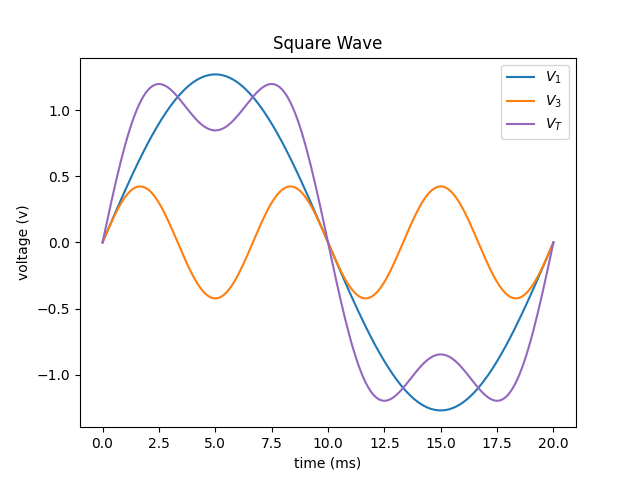
\includegraphics[width=0.784\linewidth,height=0.588\linewidth]{square-wave-3}
		\caption{$V_T:=V_T(t):=h(t \vert 2)$}
	\end{figure}
	\begin{figure}[h]\label{fig:square-wave_5}
		\centering
		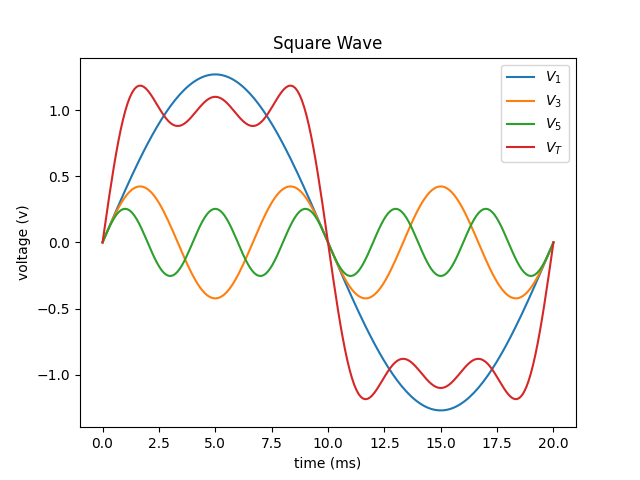
\includegraphics[width=0.784\linewidth,height=0.588\linewidth]{square-wave-5}
		\caption{$V_T:=V_T(t):=h(t \vert 3)$}
	\end{figure}
	\section[Other]{Other Non-Sinusoidal Waveforms}
	A diode only allows the current to flow in one direction.  This can have 
	the effect of distorting the AC waveform of a current produced by an AC 
	power supply.  Basically, when the value of the current would be negative, 
	which is half the duration of each cycle, it is zero instead.
	\subsection[HalfWave]{Half-wave Rectification}
	The simplest type of AC/DC rectification is half-wave, where a single diode 
	blocks half of the AC current (over time) from passing through the load. 
	(Figure below).  The supplied voltage, denoted aS '$E_T$', as a function of 
	time is given by:
	$$ E_T(t) = |E_T| \cdot \sin (2 \pi f t) \cdot u\big( \sin(2 \pi f t) \big 
	)$$
\end{document}
